\documentclass[tikz, border=4pt]{standalone}
\usepackage{tikz}
\usepackage{tikz-timing}
\begin{document}
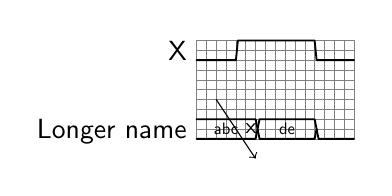
\begin{tikzpicture}[x=1cm, y=1cm]
  \node at (2.1,-0.78) {\pgfinterruptpicture%
  \begin{tikztimingtable}[timing/rowdist=4, timing/coldist=0.5]
    X & 2L 4H 2L \\
    Longer name & 3D{abc} 3D{de} 2L \\
  \extracode
    \fulltablegrid
    \draw [->] (1,-2) -- node [right] {\footnotesize x} (3,-5);
  \end{tikztimingtable}%
  \endpgfinterruptpicture};
\end{tikzpicture}
\end{document}
